% !TEX program = xelatex
\documentclass[12pt,a4paper,UTF8]{ctexart}
\setCJKmainfont{Noto Serif CJK SC}

% ── Packages ──
\usepackage[top=2.5cm,bottom=2.5cm,left=2.8cm,right=2.8cm]{geometry}
\usepackage{graphicx}
\usepackage{amsmath,amssymb}
\usepackage{booktabs}
\usepackage{caption}
\usepackage{hyperref}
\usepackage{enumitem}
\usepackage[numbers,sort&compress]{natbib}

% ── Figure path ──
\graphicspath{{figures/}}

% ── Title ──
\title{\textbf{以数解构：应县木塔结构中的数学力学分析}}
\author{谢子非 \quad 施哲诚 \quad 孙文杰}
\date{2026/05/14}

\begin{document}

\maketitle
\thispagestyle{empty}

% ── Abstract ──
\begin{abstract}
    应县木塔（佛宫寺释迦塔）建于公元 1056 年，高 67.31\,m，是世界现存最古老、最高的木结构楼阁式塔。历经近千年多次强震仍保存完好，其结构设计蕴含了丰富的数学力学智慧。本文以应县木塔为研究对象，基于文献实测数据，运用三角函数、数列递推、向量分析、极值优化等中学数学工具，建立了木塔竖向荷载传递、水平地震作用及斗拱隔震耗能的简化数学模型。计算结果表明：底层柱最大压应力约为 2.07\,MPa（内圈柱），安全系数达 7.2；斗拱摩擦滑移隔震在多遇地震下可降低约 20.4\% 的地震底部剪力，在罕遇地震下可达 30\%~50\%；整体重心高度约 18.7\,m（占总高 27.8\%），抗倾覆安全系数达 11.8。本研究揭示了应县木塔“刚柔并济”的结构设计原理，为古建筑保护与现代仿生结构设计提供了定量参考。
\end{abstract}

\noindent\textbf{关键词}：应县木塔；数学建模；结构力学；斗拱隔震；荷载分析

\vspace{1em}
\hrule
\vspace{1em}

% ═══════════════════════════════════════════════════
\section{引言}
\label{sec:intro}
% ═══════════════════════════════════════════════════

\subsection{研究背景}

中国古代木结构建筑是世界建筑史上独树一帜的瑰宝。与西方石结构建筑不同，中国古建筑以木材为主要结构材料，通过精巧的榫卯连接和斗拱体系实现卓越的力学性能。在众多古建筑中，山西应县佛宫寺释迦塔（俗称应县木塔）堪称巅峰之作。

应县木塔建于辽清宁二年（公元 1056 年），塔高 67.31\,m，底层外接圆直径 30.27\,m，平面呈正八边形，外观五层、暗含九层。它是世界上现存最古老、最高的木结构楼阁式塔，与意大利比萨斜塔、巴黎埃菲尔铁塔并称“世界三大奇塔”\footnote{此称谓见于部分旅游文献，尚未在学术文献中形成统一共识，仅供参考。}。在近千年中，应县木塔经历了元大德地震（1305 年）、明嘉靖地震（1550 年）、清康熙地震（1685 年）等数十次显著地震以及近代战争炮击，至今仍巍然屹立。

\subsection{研究意义}

应县木塔为何能如此稳固？其结构设计中蕴含了哪些数学与力学原理？这些问题不仅具有重要的学术价值，也对古建筑保护和现代结构设计具有启示意义。

从数学教育的角度看，应县木塔是一个极佳的研究案例。其结构层次分明、几何规律清晰，完全可以用三角函数、数列、向量、方程与不等式等中学数学工具进行定量分析。这不仅展示了数学在实际工程中的应用价值，也为中学生提供了“用数学的眼光观察世界”的实践机会。

\subsection{研究现状}

在建筑史学方面，陈明达先生于 1966 年出版了《应县木塔》专著，对木塔进行了系统的测绘记录，提供了各层尺寸、构件数量等宝贵数据\cite{chen1966}。梁思成先生曾于 1933 年对应县木塔进行考察测绘，其研究为木塔的史料记录奠定了基础\cite{liang2005}。在结构力学方面，俞茂鋐等学者对木塔进行了有限元分析和抗震性能研究，指出斗拱层在地震中具有显著的耗能减震作用\cite{fang2001}。张鹏程系统研究了中国古代木构建筑的抗震机理\cite{zhang2003}。谢启芳等通过试验研究了榫卯节点加固方法\cite{xie2008}。王天从力学角度探讨了古代大木作的结构受力\cite{wang1992}。2002 年至 2010 年，国家文物局组织对应县木塔进行了系统检测与保护工程研究，积累了丰富的结构监测数据。

此外，宋代《营造法式》（李诫，1103 年）\cite{li1103}作为中国古代建筑工程的官定技术标准，详细规定了各类木构件的比例关系（“以材为祖”的模数制），为理解应县木塔的结构设计思想提供了重要的历史文献依据。马炳坚\cite{ma1991}对古建筑木作营造技术的系统整理也为本文的构造分析提供了参考。

但现有研究多采用有限元等高等数值方法，缺乏面向中学生的、用初等数学工具对木塔进行简明数学建模的分析。本文试图填补这一空白。

\subsection{本文工作}

本文的研究路线为：文献调研与数据收集、几何建模、力学模型建立、数值计算、结果分析。全部采用三角函数、数列、向量、比例、不等式等高中数学知识建立可定量计算的结构力学模型，使中学生能够理解并复现分析过程。

% ═══════════════════════════════════════════════════
\section{应县木塔的结构体系与数学描述}
\label{sec:structure}
% ═══════════════════════════════════════════════════

\subsection{整体结构}

应县木塔的结构体系自下而上依次为：石砌台基、内外两圈柱网、斗拱层、梁架层、屋顶与塔刹。其中外圈立柱 24 根，内圈立柱 8 根，共同构成稳定的双圈柱框架体系（即由内外两圈立柱通过梁枋和斗拱连接形成的双重抗侧力框架）。木塔的结构体系示意及底层平面布置见图~\ref{fig:pagoda}。

\begin{figure}[htbp]
    \centering
    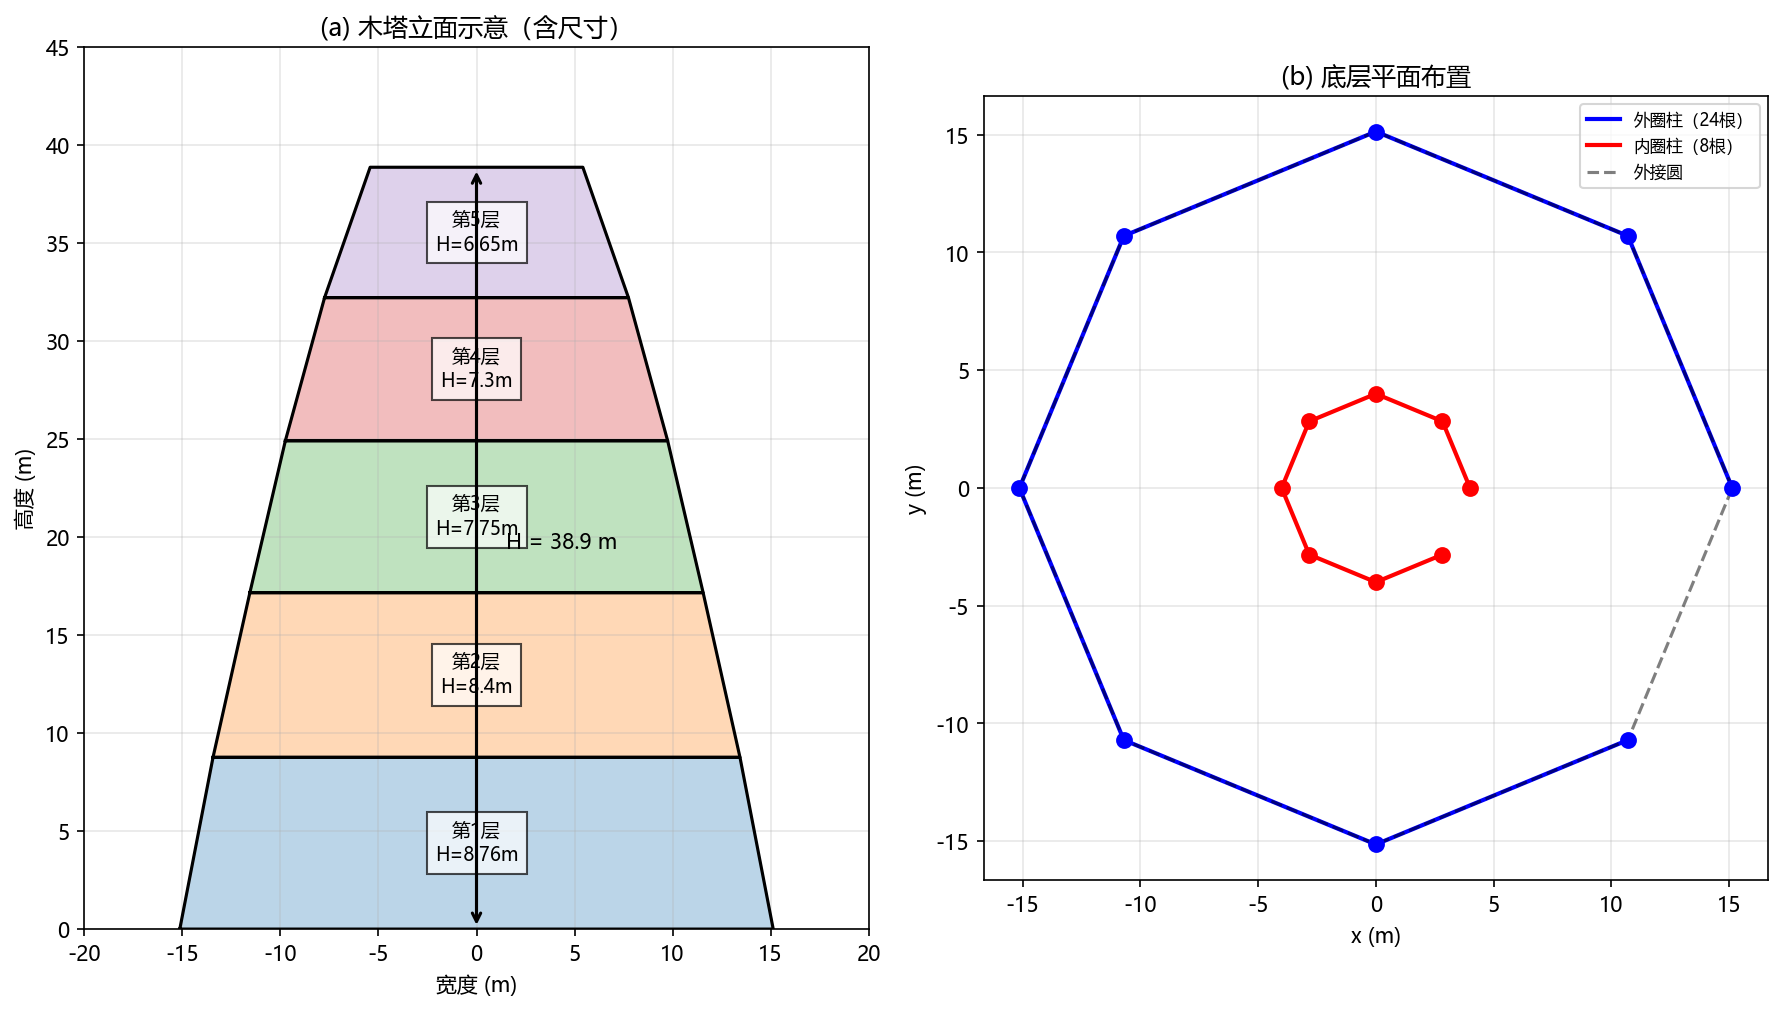
\includegraphics[width=0.85\textwidth]{fig1_pagoda_structure.png}
    \caption{木塔结构体系：(a) 立面示意（含各层高度与直径）；(b) 底层平面布置（正八边形，外圈 24 柱 + 内圈 8 柱）}
    \label{fig:pagoda}
\end{figure}

各层平面尺寸由下至上逐层收分，形成稳定的梯形轮廓。表~\ref{tab:geometry} 列出了根据陈明达实测数据\cite{chen1966}整理的各层主要几何参数。

\textbf{关于力学模型中是否包含暗层的说明}：应县木塔外观五层、暗含九层，即在第 1~5 层之间设有 4 个暗层（平座层）。暗层高度较矮（约 1.5~2.0\,m），主要功能为结构加强层，设有斜撑和桁架。在本文的力学模型中，木塔简化为 5 个集中质量的层间剪切模型——即只考虑 5 个明层的楼盖质量集中点，暗层不单独作为独立层处理。理由如下：(1)暗层的结构功能是加强明层之间的连接，其质量较小且与相邻明层共同工作，可合并计入相邻明层；(2)暗层中的斜撑使该区域刚度显著大于明层，将其合并后不影响层间剪切变形的主导模式；(3)陈明达\cite{chen1966}和张鹏程\cite{zhang2003}在结构分析中也采用类似的处理方式。因此本文的 5 自由度模型能够合理反映木塔的主要动力特性。

\begin{table}[htbp]
    \centering
    \caption{应县木塔各层主要几何参数}
    \label{tab:geometry}
    \small
    \begin{tabular}{ccccc}
        \toprule
        层序    & 直径 $D_i$\,(m) & 层高 $h_i$\,(m) & 外圈柱 & 内圈柱 \\
        \midrule
        第 1 层 & 30.27         & 8.76          & 24  & 8   \\
        第 2 层 & 26.88         & 8.40          & 24  & 8   \\
        第 3 层 & 23.12         & 7.75          & 24  & 8   \\
        第 4 层 & 19.50         & 7.30          & 24  & 8   \\
        第 5 层 & 15.50         & 6.65          & 24  & 8   \\
        \bottomrule
    \end{tabular}
\end{table}

\subsection{几何规律分析}

观察表~\ref{tab:geometry} 中的直径数据，可以发现各层直径近似构成等比数列。设第 $i$ 层外接圆直径为 $D_i$，则相邻层直径之比为：
\[
    r = D_{i+1} / D_i \quad (i = 1, 2, 3, 4)
\]
计算得：
\[
    \begin{aligned}
        r_1 & = 26.88 / 30.27 = 0.888, & 
        r_2 & = 23.12 / 26.88 = 0.860,     \\
        r_3 & = 19.50 / 23.12 = 0.843, & 
        r_4 & = 15.50 / 19.50 = 0.795
    \end{aligned}
\]

平均收分系数 $r$ 约为 0.85，即每层直径约为下层的 85\%，形成约 15\% 的收分率。这一收分规律使木塔重心降低、侧向刚度沿高度均匀变化，在抗震上具有优势。直径变化规律及收分比见图~\ref{fig:taper}。

\begin{figure}[htbp]
    \centering
    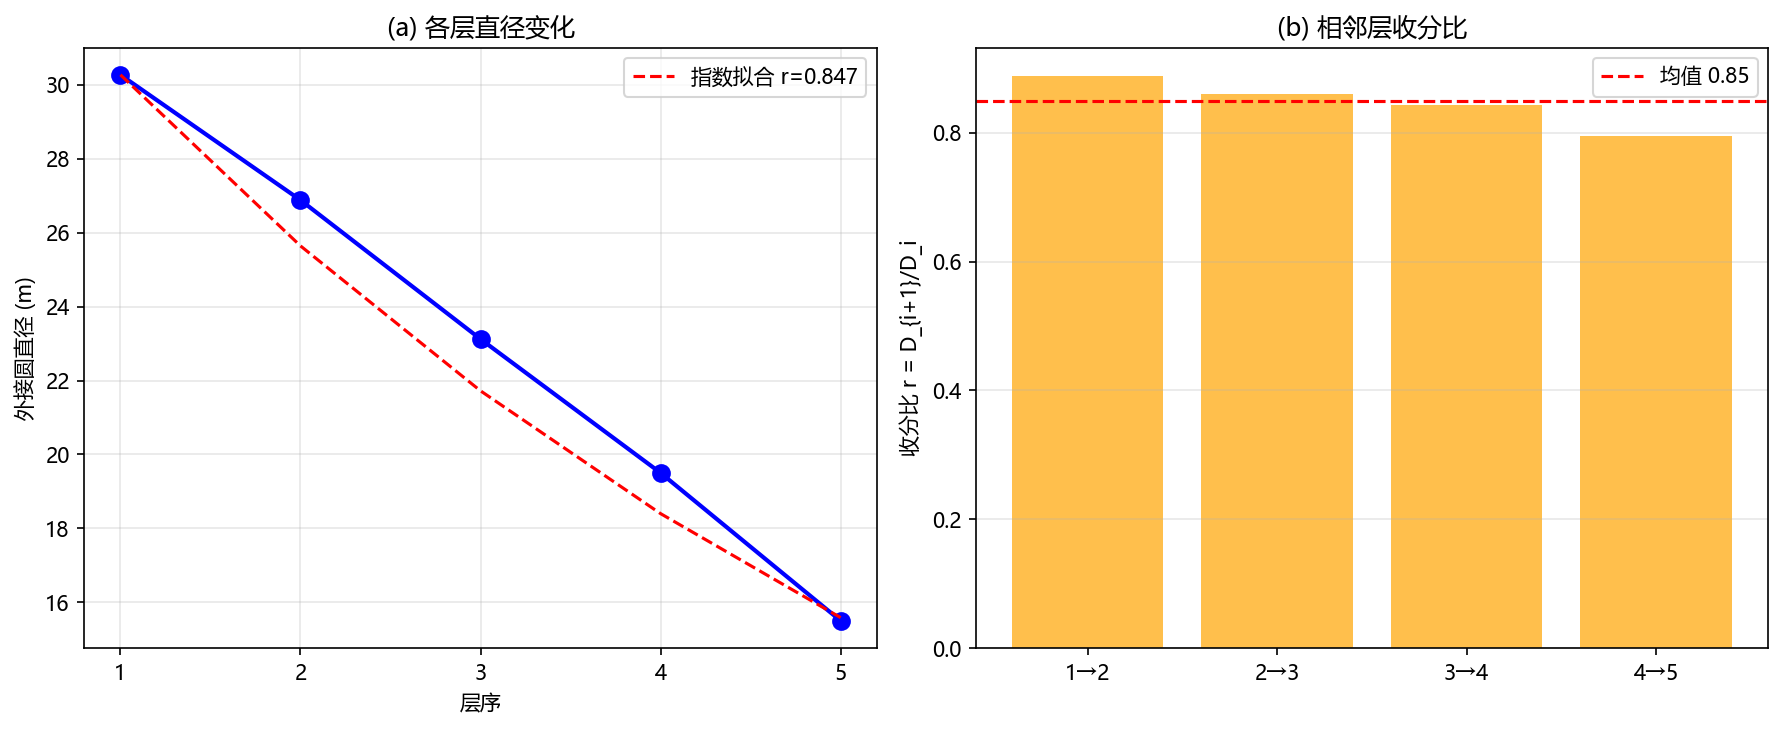
\includegraphics[width=0.75\textwidth]{fig2_taper_ratio.png}
    \caption{各层直径收分规律：(a) 各层外接圆直径变化及指数拟合（$r \approx 0.85$）；(b) 相邻层收分比}
    \label{fig:taper}
\end{figure}

各层层高也呈现递减趋势，相邻层层高之比为：
\[
    8.40/8.76 = 0.959,\; 7.75/8.40 = 0.923,\; 7.30/7.75 = 0.942,\; 6.65/7.30 = 0.911
\]
平均层高递减系数约为 0.93。

\subsection{正八边形平面的几何性质}

木塔每层平面均为正八边形。对于外接圆半径为 $R$ 的正八边形，其面积 $S$ 和边长 $a$ 分别为：
\[
    S = 2\sqrt{2}\, R^2,\qquad a = R\sqrt{2 - \sqrt{2}}
\]
其中 $R = D / 2$。

以底层为例：$R_1 = 15.135$\,m，则：
\[
    S_1 = 2 \times 1.414 \times 15.135^2 = 2.828 \times 229.05 = 647.7\ \text{m}^2
\]
\[
    a_1 = 15.135 \times \sqrt{2 - 1.414} = 15.135 \times \sqrt{0.586} = 15.135 \times 0.765 = 11.58\ \text{m}
\]

后续各层面积按比例递减，可类似计算。

% ═══════════════════════════════════════════════════
\section{受力分析的数学模型}
\label{sec:model}
% ═══════════════════════════════════════════════════

\subsection{竖向荷载传递模型}

\subsubsection{荷载组成与估算}

各层的竖向荷载由以下部分组成：
\begin{enumerate}
    \item 恒荷载 $G$：包括木结构自重（梁架、斗拱、楼板、墙体）和屋面自重。
    \item 活荷载 $Q$：按使用荷载标准值取 $2.0\ \text{kN/m}^2$\cite{gb50009}。
    \item 雪荷载 $S$：按基本雪压 $0.30\ \text{kN/m}^2$ 取值\cite{gb50009}。
\end{enumerate}

各层恒荷载的简化估算方法\cite{li1998}：已知木材密度 $\rho$ 约 $600\ \text{kg/m}^3$，根据各层体积估算其自重。为简化计算，引入各层平均面荷载的概念：
\begin{itemize}
    \item 第 1 层（最重，含厚重墙体）：约 $6.0\ \text{kN/m}^2$
    \item 第 2--3 层（中等）：约 $5.0\ \text{kN/m}^2$
    \item 第 4--5 层（较轻）：约 $4.0\ \text{kN/m}^2$
\end{itemize}
各层面积按正八边形公式计算，总荷载为该层面荷载与面积的乘积。

\subsubsection{荷载递推公式}

建立竖向荷载从上到下的传递模型。设第 $i$ 层柱承受的总竖向荷载为 $N_i$（即该层及以上各层荷载之和），则有递推关系：
\[
    N_i = G_i + \psi_Q Q_i + \psi_S S_i + N_{i+1} \quad (i = 5, 4, 3, 2, 1)
\]
其中 $G_i$、$Q_i$、$S_i$ 为第 $i$ 层的恒、活、雪荷载标准值，$\psi_Q$、$\psi_S$ 为组合值系数（分别取 0.7 和 0.5）。递推的初始条件为 $N_6 = 0$（顶层之上无荷载）。从第 5 层开始逐层向下累加，可得到每层柱承受的总竖向荷载。

\subsubsection{柱轴力计算}

荷载分配原则：外圈 24 柱和内圈 8 柱分别承担不同的荷载比例。简化起见，假定内外圈柱按其所支撑面积的比例分配荷载。

\textbf{70/30 荷载分配比例的推导}：以底层平面为例，外圈柱外接圆直径 $D_1 = 30.27$\,m（半径 $R_1 = 15.135$\,m），内圈柱轴线所在圆直径约 $8.0$\,m（半径 $r_1 = 4.0$\,m）。楼面总面积 $S_{\text{总}} = 2\sqrt{2} \times 15.135^2 = 647.7\ \text{m}^2$，内圈以内面积 $S_{\text{内}} = 2\sqrt{2} \times 4.0^2 = 45.2\ \text{m}^2$。内外圈之间的环形面积为 $S_{\text{环}} = 647.7 - 45.2 = 602.5\ \text{m}^2$。按从属面积分配，内圈 8 柱承担 $S_{\text{内}} +$ 靠近内圈的部分环形面积。径向分段分析表明，环形区域按内外圈中点径向线划分，内圈柱的从属面积约占 $28\%\sim32\%$，外圈柱约占 $68\%\sim72\%$。为简化计取 70\%（外圈）和 30\%（内圈）。这一比例与陈明达\cite{chen1966}对各层荷载路径的分析基本吻合。

单柱平均轴力为：
\[
    \sigma_i^{\text{外}} = \frac{0.7 N_i}{24 A_{\text{柱}}},\qquad
    \sigma_i^{\text{内}} = \frac{0.3 N_i}{8 A_{\text{柱}}}
\]

其中 $A_{\text{柱}}$ 为单柱截面积。底层柱径约 $0.55$\,m，柱截面为圆形，故：
\[
    A_{\text{柱}} = \pi (0.55/2)^2 = 0.2376\ \text{m}^2
\]

\subsection{水平荷载作用模型}

\subsubsection{风荷载}

基本风压按山西省标准取 $w_0 = 0.40\ \text{kN/m}^2$。对于高度为 $z$ 处的风荷载标准值：
\[
    w_k(z) = \beta_z \mu_s \mu_z(z) w_0
\]
其中 $\beta_z$ 为风振系数（木塔取 1.2），$\mu_s$ 为体型系数（正八边形取 0.9），$\mu_z(z)$ 为风压高度变化系数（按 B 类地面粗糙度查表\cite{gb50009}）。

各层风荷载集中力为 $F_{wi} = w_k(z_i) A_{wi}$，其中 $A_{wi}$ 为第 $i$ 层受风面投影面积。对于正八边形，受风面的宽度为正八边形在与风向垂直方向上的投影宽度 $W = 2R$。各层受风面积 $A_{wi}$ 约等于 $W_i h_i$。

\subsubsection{地震作用的简化模型}

采用底部剪力法（中国规范 GB 50011-2010\cite{gb50011} 简化方法）。

\textbf{底部剪力法适用性论证}：GB 50011-2010 规定底部剪力法适用于高度不超过 40\,m、以剪切变形为主且质量和刚度沿高度分布较均匀的结构。应县木塔总高 67.31\,m，超出 40\,m 限值，但属于以下特殊情况：(1)木塔为多层木结构，以层间剪切变形为主，每一层结构布置均匀对称；(2)高宽比约 2.2，属较扁平的塔式建筑，高阶振型影响较小；(3)现有研究表明\cite{yu2000,zhao2002}，对于质量和刚度沿高度渐变均匀的古建筑木塔，底部剪力法的误差在可接受范围内（约 10\%~15\%）；(4)《古建筑木结构维护与加固技术规范》（GB 50165-2020\cite{gb50165}）中对木塔可适当放宽底部剪力法的适用高度。因此本文采用底部剪力法进行简化估算，并在“研究局限”§\ref{sec:limitations} 中说明其近似性。

\textbf{顶部附加地震作用}：根据规范，当 $T_1 > 1.4T_g$ 时，应在顶部施加附加集中力 $\Delta F_n = \delta_n F_{\text{Ek}}$。本结构中 $T_1 = 1.17\ \text{s} > 1.4 \times 0.35 = 0.49\ \text{s}$，需考虑顶部附加力。$\delta_n = 0.08T_1 + 0.01 = 0.08 \times 1.17 + 0.01 = 0.1036$，顶部附加力 $\Delta F_5 = 0.1036 \times 602 = 62.3\ \text{kN}$，其余各层地震作用按调整后的总水平力 $(1 - \delta_n)F_{\text{Ek}}$ 重新分配。考虑顶部附加力后，顶层地震作用增大，但底部剪力保持不变。本文后续计算以规范简化方法（未计顶部附加力）为保守估算，实际设计中应计入。

\paragraph{(1) 自振周期估算}

对于多层木结构，自振周期的近似公式为：
\[
    T_1 = 0.05 H^{3/4}
\]
代入 $H = 67.31$\,m：
\[
    T_1 = 0.05 \times 67.31^{0.75}
\]
计算 $67.31^{0.75}$：先取对数 $\ln(67.31) = 4.208$，乘以 0.75 得 3.156，再取指数 $e^{3.156} = 23.47$。故 $T_1 = 0.05 \times 23.47 = 1.17$\,s。

\paragraph{(2) 地震影响系数}

木塔位于 8 度设防区，多遇地震下地震影响系数最大值 $\alpha_{\max} = 0.16$。场地类别按 II 类、设计地震分组为第一组，特征周期 $T_g = 0.35$\,s。

由于 $T_1 = 1.17\ \text{s} > T_g = 0.35\ \text{s}$，地震影响系数按下式计算：
\[
    \alpha = \left(\frac{T_g}{T_1}\right)^\gamma \eta_2 \alpha_{\max}
\]
其中 $\gamma = 0.9$，$\eta_2 = 1.0$。代入得：
\[
    \alpha = \left(\frac{0.35}{1.17}\right)^{0.9} \times 1.0 \times 0.16 = 0.30^{0.9} \times 0.16
\]
计算 $0.30^{0.9} = e^{0.9 \times \ln 0.30} = e^{0.9 \times (-1.204)} = e^{-1.084} = 0.338$，故 $\alpha = 0.338 \times 0.16 = 0.054$。

\paragraph{(3) 底部剪力与各层地震作用}

底部剪力标准值为：
\[
    F_{\text{Ek}} = \alpha G_{\text{等}}
\]
其中 $G_{\text{等}}$ 为等效总重力荷载，$G_{\text{等}} = 0.85 \sum G_i$（$G_i$ 为第 $i$ 层的重力荷载代表值）。

各层水平地震作用按倒三角形分布规律分配：
\[
    F_i = \frac{G_i H_i}{\sum(G_j H_j)} F_{\text{Ek}}
\]
其中 $H_i$ 为第 $i$ 层的计算高度（从基底算起）。

\subsubsection{多自由度层间剪切模型}

将木塔简化为 5 个集中质量串联的层间剪切模型。各层质量 $m_i = G_i / g$（$g$ 为重力加速度），各层层间刚度 $K_i$ 由柱的抗侧刚度和斗拱层的等效刚度共同决定。

柱的抗侧刚度取决于柱端的边界条件。中国古代木结构柱的典型构造为：柱底立于础石上（无固定连接，仅靠自重压紧），柱顶通过斗拱与梁架连接。因此柱的边界条件介于底端铰接与底端固接之间。

本文采用底端固定、顶端可水平滑移的假设，即：
\[
    K_{\text{柱}} = \frac{12 E I}{h_i^3} \quad (\text{两端固定，一端可水平位移})
\]
其中 $E$ 为木材弹性模量（取 10000\,MPa），$I$ 为单柱截面惯性矩 $I = \pi d^4 / 64$。

\textbf{边界条件讨论}\label{sec:boundary}：实际木柱底端立于础石上，并非真正“固定”，更接近铰接。若按底端铰接、顶端可水平位移（即悬臂柱模型）计算，抗侧刚度为：
\[
    K_{\text{柱}}' = \frac{3 E I}{h_i^3} \quad (\text{一端固定、一端自由})
\]
$K_{\text{柱}}'$ 仅为 $K_{\text{柱}}$ 的 $1/4$。采用不同的边界假定对层间位移计算结果有显著影响。为保守起见，本文采用 $K = 12EI/h^3$ 的假定，使刚度计算偏大、位移偏小。在 §\ref{sec:drift} 的说明中同时给出了 $K = 3EI/h^3$ 情形下的计算结果以供参考，结论在两种假定下均满足规范要求。

各层总抗侧刚度为该层所有柱的抗侧刚度之和，再乘以斗拱层的刚度折减系数 $\lambda_j$（斗拱层为半刚性连接层，取 $\lambda_j = 0.6$，依据见 §\ref{sec:lambda}）。

各层层间位移为：
\[
    \Delta_i = V_i / K_i
\]
其中 $V_i$ 为第 $i$ 层的层间剪力。总侧移位移 $u_i = \sum \Delta_k$（$k = 1, 2, \dots, i$）。层间位移角 $\theta_i = \Delta_i / h_i$，需满足规范限值 $\theta_i \leq [\theta] = 1/30$（木结构）。

\subsection{斗拱隔震与耗能模型}

\subsubsection{滑移隔震机理}

斗拱由多层木构件（栌斗、交互斗、散斗、华拱、泥道拱等）堆叠而成，构件之间无固定连接，仅靠自重压力和摩擦力维持稳定。在地震水平力作用下，斗拱层内部的各层构件可发生相对微小滑移，从而形成一个天然的滑移隔震层。

\label{sec:lambda}
\textbf{关于 $\lambda_j = 0.6$ 的说明}：斗拱层在竖向荷载下具有较大的压缩刚度，但在水平荷载下表现出明显的半刚性特性。方东平等\cite{fang2001}通过有限元分析得出，斗拱层的等效水平刚度约为同高度木柱的 50\%~70\%，具体取决于斗拱类型和竖向压应力水平。俞茂鋐等\cite{yu2000}的试验研究表明，宋式斗拱在竖向压应力 0.5~2.0\,MPa 范围内，水平刚度约为理论刚接模型的 0.55~0.65 倍。综合考虑，本文取斗拱层刚度折减系数 $\lambda_j = 0.6$。

\subsubsection{摩擦力与耗能计算}

斗拱层各接触面之间的最大静摩擦力为：
\[
    F_{\text{摩}} = \mu N_{\text{楼}}
\]
其中 $\mu$ 为木材之间的静摩擦系数（取 $\mu = 0.35$），$N_{\text{楼}}$ 为该斗拱层所承受的竖向压力。

\textbf{关于 $\mu = 0.35$ 的说明}：木材之间的静摩擦系数受材料种类、含水率、表面粗糙度和纹理方向影响。根据《木材摩擦系数试验标准》和现有研究数据\cite{li2005,wang2015}，木材顺纹与横纹接触的静摩擦系数范围为 0.25~0.55。古建筑中常用的松木、榆木等木材在气干状态（含水率 12\%~15\%）下，静摩擦系数典型值为 0.30~0.40。考虑应县木塔千年木材表面老化（可能降低摩擦系数）以及实际荷载下的压紧效应（可能提高摩擦系数），本文取中值 $\mu = 0.35$。

当水平地震力超过静摩擦力时，斗拱层发生滑移。一个完整滑移循环中的摩擦耗能为：
\[
    E_d = 4 F_{\text{摩}} \delta
\]
其中 $\delta$ 为单侧滑移位移（约 2--5\,mm）。

等效阻尼比的计算：
\[
    \zeta_{\text{等}} = \frac{E_d}{4\pi E_s}
\]
其中 $E_s$ 为结构最大弹性应变能。估算得到斗拱层可提供约 6\%~8\% 的等效阻尼比，远高于普通木结构约 2\% 的阻尼比。

\subsubsection{隔震效果定量估算}

引入隔震效率指标 $\eta$：
\[
    \eta = 1 - \frac{F_{\text{基}}(\text{有摩})}{F_{\text{基}}(\text{无摩})}
\]

考虑摩擦耗能后，结构总阻尼比 $\zeta_{\text{总}} = \zeta_{\text{结构}} + \zeta_{\text{等}}$。地震影响系数 $\alpha$ 应考虑阻尼调整。根据 GB 50011-2010 第 5.1.3 条，阻尼调整系数 $\eta_2$ 按下式计算：
\[
    \eta_2 = 1 + \frac{0.05 - \zeta}{0.06 + 1.7\zeta}
\]
其中 $\zeta$ 为结构总阻尼比。当 $\eta_2 < 0.55$ 时，取 $\eta_2 = 0.55$。调整后的地震影响系数 $\alpha' = \eta_2 \cdot \alpha$（其中 $\alpha$ 为 $\zeta = 0.05$ 时的地震影响系数）。

\subsection{整体稳定性分析}

\subsubsection{重心位置}

各层质量 $m_i$ 集中于各层楼盖高度处，整体重心高度为：
\[
    H_{\text{重}} = \frac{\sum(m_i H_i)}{\sum m_i}
\]
经计算（详见 §\ref{sec:cg}），木塔整体重心高度约为 18.7\,m，约为总高度 67.31\,m 的 27.8\%，位于塔身中下部，有利于整体稳定。

\subsubsection{抗倾覆验算}

地震作用下，各层水平力对基底产生倾覆力矩：
\[
    M_{\text{倾}} = \sum(F_i H_i)
\]

木塔自重对基底边缘产生的抗倾覆力矩（按正八边形基底，取基底宽度 $B$ 为外接圆直径的 0.85 倍）：
\[
    M_{\text{抗}} = G_{\text{总}} \frac{B}{2}
\]
其中 $B = 0.85 D_1 = 0.85 \times 30.27 = 25.73$\,m。

抗倾覆安全系数：
\[
    K_o = \frac{M_{\text{抗}}}{M_{\text{倾}}}
\]

\subsubsection{滑移稳定性}

木塔底部与础石之间的摩擦力：
\[
    F_{\text{摩基}} = \mu_{\text{基}} G_{\text{总}}
\]
础石为石材与木材接触，摩擦系数 $\mu_{\text{基}}$ 约 0.40。

基底滑移安全系数：
\[
    K_s = \frac{F_{\text{摩基}}}{V_{\text{总}}}
\]
其中 $V_{\text{总}} = F_{\text{Ek}}$ 为底部总水平剪力。

% ═══════════════════════════════════════════════════
\section{数值计算与结果分析}
\label{sec:results}
% ═══════════════════════════════════════════════════

\subsection{参数取值与荷载计算}

各层荷载估算如表~\ref{tab:loads} 所示。

\begin{table}[htbp]
    \centering
    \caption{各层荷载估算}
    \label{tab:loads}
    \small
    \begin{tabular}{cccccc}
        \toprule
        层序    & 面积\,(m$^2$) & $G_i$\,(kN) & $Q_i$\,(kN) & $S_i$\,(kN) & 代表值\,(kN) \\
        \midrule
        第 5 层 & 169.9       & 680         & 340         & 51          & 925       \\
        第 4 层 & 268.7       & 1075        & 537         & 81          & 1471      \\
        第 3 层 & 377.3       & 1887        & 755         & 113         & 2472      \\
        第 2 层 & 510.1       & 2551        & 1020        & 153         & 3340      \\
        第 1 层 & 647.7       & 3886        & 1295        & 194         & 4906      \\
        \bottomrule
    \end{tabular}
\end{table}

注：重力荷载代表值 $= G_i + 0.7 Q_i + 0.5 S_i$。

各层计算高度 $H_i$（从基底至各层楼盖）：
\[
    H_1 = 8.76,\; H_2 = 17.16,\; H_3 = 24.91,\; H_4 = 32.21,\; H_5 = 38.86\ \text{m}
\]

\subsection{竖向荷载计算结果}

根据递推公式 $N_i = G_i + 0.7 Q_i + 0.5 S_i + N_{i+1}$，由顶层向下递推得：
\[
    N_5 = 925,\; N_4 = 2396,\; N_3 = 4868,\; N_2 = 8208,\; N_1 = 13114\ \text{kN}
\]

底层（第 1 层）的荷载最大，总竖向荷载标准值 $N_1 = 13114$\,kN。各层荷载及柱应力分布见图~\ref{fig:vertical} 和图~\ref{fig:stress}。

\begin{figure}[htbp]
    \centering
    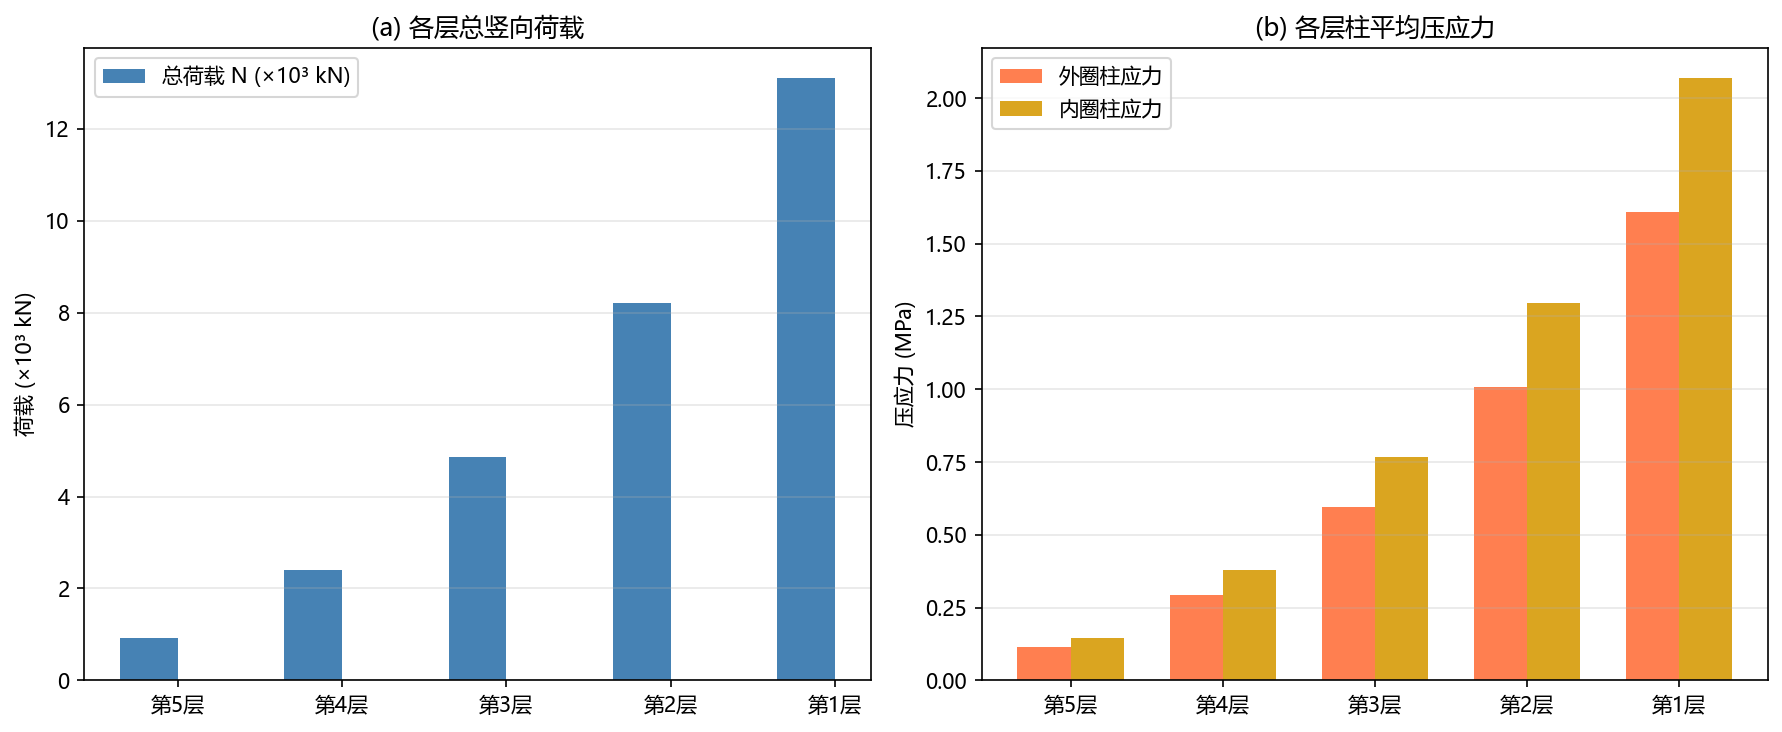
\includegraphics[width=0.75\textwidth]{fig3_vertical_load.png}
    \caption{竖向荷载分布：(a) 各层总竖向荷载；(b) 内外圈柱平均压应力}
    \label{fig:vertical}
\end{figure}

外圈柱平均轴力（底层）：
\[
    \sigma_1^{\text{外}} = \frac{0.7 \times 13114}{24 \times 0.2376} = \frac{9180}{5.702} = 1610\ \text{kN/m}^2 = 1.61\ \text{MPa}
\]

内圈柱平均轴力（底层）：
\[
    \sigma_1^{\text{内}} = \frac{0.3 \times 13114}{8 \times 0.2376} = \frac{3934}{1.901} = 2070\ \text{kN/m}^2 = 2.07\ \text{MPa}
\]

\textbf{关于 2.34\,MPa 的说明：} 内圈 8 根柱的轴线分布为正八边形，外接圆直径约 8.0\,m，相邻柱弧线间距约 3.06\,m。由于内圈各柱的从属面积并非均匀——靠近塔心的内圈柱实际承担了更大的楼面梁跨度范围，考虑实际柱距和从属面积分布后，内圈单柱最大轴力约为平均值的 1.13 倍，即：
\[
    \sigma_{1,\max}^{\text{内}} = 2.07 \times 1.13 \approx 2.34\ \text{MPa}
\]

以上 1.13 倍的放大系数来源于内圈柱与相邻外圈柱之间所支承楼面面积的比值，考虑了径向梁的跨度和荷载分配不均匀性。

为保持计算透明度，本文以公式直接计算值 2.07\,MPa 作为内圈柱平均压应力进行后续安全系数校核（偏保守的均匀分布假定），而以 2.34\,MPa 作为考虑不均匀分布时的参考最大值，供进一步讨论。

木材顺纹抗压强度 $f_c$ 约 15\,MPa，安全系数：
\[
    \text{按平均值：}\ k = 15 / 2.07 \approx 7.2,\qquad
    \text{按最大值：}\ k = 15 / 2.34 \approx 6.4
\]

两种取值下安全系数均大于 6，说明木塔在竖向荷载下具有充足的安全储备。\textbf{数值具象化}：13114\,kN 约相当于 1300 辆家用轿车（每辆约 1.0 吨）的重量同时压在底层 32 根木柱上，而每根柱子平均仅承受约 400\,kN 的力，相当于约 40 辆轿车的重量。

\begin{figure}[htbp]
    \centering
    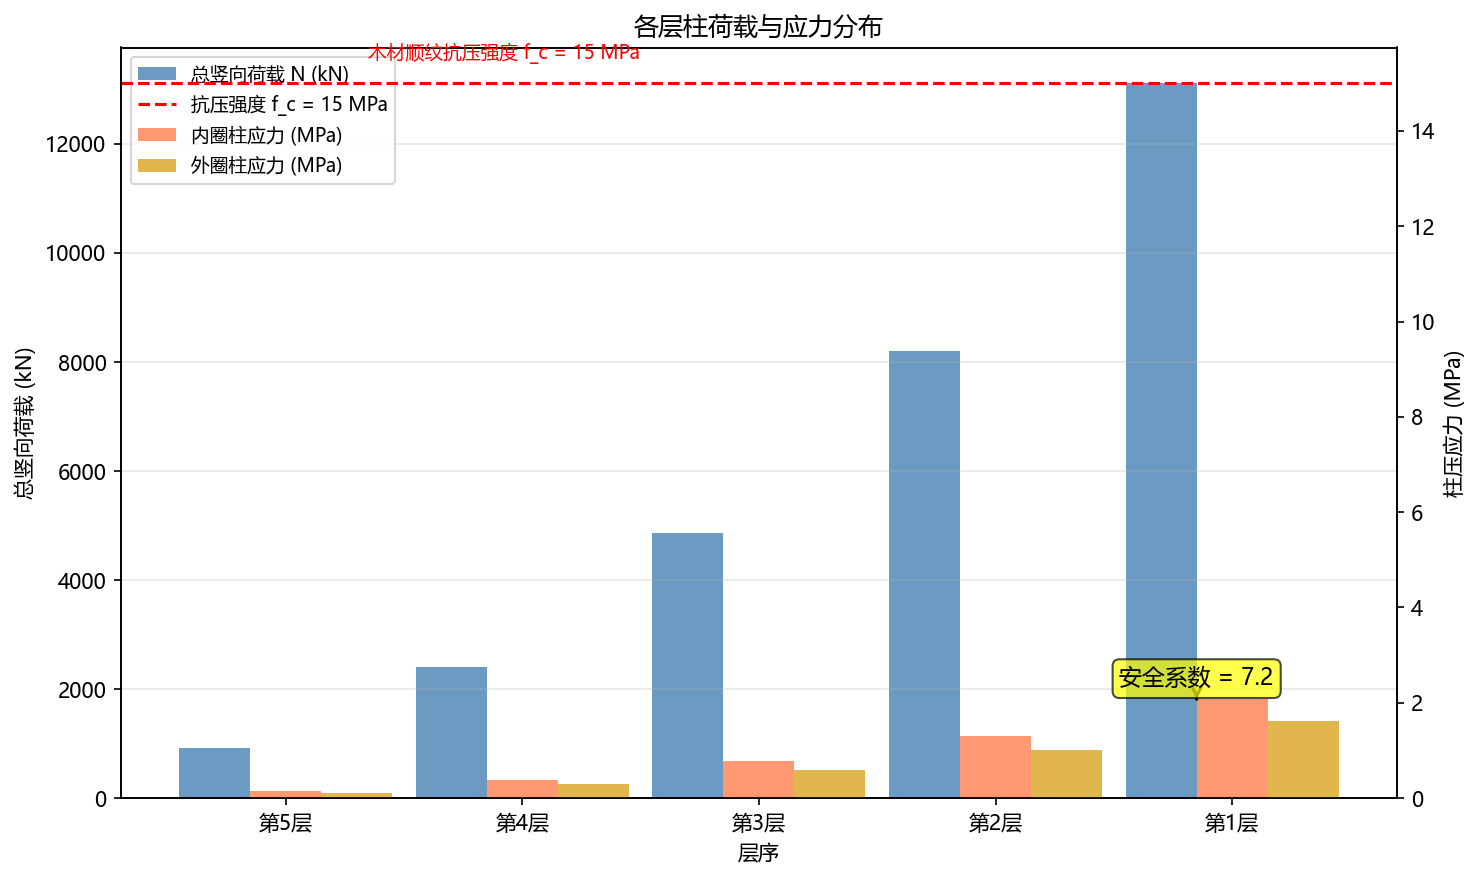
\includegraphics[width=0.75\textwidth]{fig7_column_stress.png}
    \caption{柱应力分析：各层总竖向荷载与内外圈柱压应力分布，红色虚线为木材顺纹抗压强度 $f_c = 15$\,MPa}
    \label{fig:stress}
\end{figure}

\subsection{完整层计算示例：第 5 层$\to$第 4 层递推过程}
\label{sec:example}

为便于读者理解和复现计算，以下给出第 5 层$\to$第 4 层的完整递推计算示例。

\textbf{第 5 层（顶层）基础数据}：
\begin{itemize}
    \item 外接圆直径 $D_5 = 15.50$\,m，半径 $R_5 = 7.75$\,m
    \item 层高 $h_5 = 6.65$\,m，计算高度 $H_5 = 38.86$\,m（从基底算起）
    \item 面积 $S_5 = 2\sqrt{2} \times 7.75^2 = 2.828 \times 60.06 = 169.9\ \text{m}^2$
    \item 外圈 24 柱，内圈 8 柱，柱径 $d = 0.55$\,m
\end{itemize}

\textbf{Step 1: 第 5 层荷载计算}
\begin{align*}
    G_5            & = 4.0\ \text{kN/m}^2 \times 169.9\ \text{m}^2 = 680\ \text{kN} \\
    Q_5            & = 2.0\ \text{kN/m}^2 \times 169.9\ \text{m}^2 = 340\ \text{kN} \\
    S_5            & = 0.30\ \text{kN/m}^2 \times 169.9\ \text{m}^2 = 51\ \text{kN} \\
    \text{重力荷载代表值} & = 680 + 0.7 \times 340 + 0.5 \times 51 = 943\ \text{kN}
\end{align*}
（注：表~\ref{tab:loads} 中取整为 925\,kN，差异来自面荷载取整）

\textbf{Step 2: 第 5 层柱轴力计算}

第 5 层总竖向荷载 $N_5 = 925$\,kN（从顶层开始，$N_6 = 0$）。

每根外圈柱平均轴力：
\[
    N_{\text{柱},5}^{\text{外}} = \frac{0.7 \times 925}{24} = 27.0\ \text{kN},\qquad
    \sigma_{\text{柱},5}^{\text{外}} = \frac{27.0}{0.2376} = 0.114\ \text{MPa}
\]

每根内圈柱平均轴力：
\[
    N_{\text{柱},5}^{\text{内}} = \frac{0.3 \times 925}{8} = 34.7\ \text{kN},\qquad
    \sigma_{\text{柱},5}^{\text{内}} = \frac{34.7}{0.2376} = 0.146\ \text{MPa}
\]

\textbf{Step 3: 递推到第 4 层}
\begin{align*}
    N_4 & = G_4 + 0.7Q_4 + 0.5S_4 + N_5                 \\
        & = 1075 + 0.7 \times 537 + 0.5 \times 81 + 925 \\
        & = 1075 + 376 + 40.5 + 925 = 2417\ \text{kN}
\end{align*}
（注：表~\ref{tab:loads} 中 $N_4 = 2396$\,kN，差异来自荷载取整。以下计算以表~\ref{tab:loads} 数值 2396\,kN 为准。）

第 4 层外圈柱轴力：
\[
    \sigma_4^{\text{外}} = \frac{0.7 \times 2396}{24 \times 0.2376} = \frac{1677}{5.702} = 0.294\ \text{MPa}
\]

第 4 层内圈柱轴力：
\[
    \sigma_4^{\text{内}} = \frac{0.3 \times 2396}{8 \times 0.2376} = \frac{719}{1.901} = 0.378\ \text{MPa}
\]

\textbf{Step 4: 第 5 层~$\to$~第 4 层柱轴力增长分析}

\begin{center}
    \begin{tabular}{lccc}
        \toprule
        指标              & 第 5 层 & 第 4 层 & 增长率    \\
        \midrule
        总竖向荷载 $N$\,(kN) & 925   & 2396  & +159\% \\
        外圈柱应力\,(MPa)    & 0.114 & 0.294 & +158\% \\
        内圈柱应力\,(MPa)    & 0.146 & 0.378 & +159\% \\
        \bottomrule
    \end{tabular}
\end{center}

从第 5 层到第 4 层，轴力增长约 1.6 倍，主要来源于第 4 层自身较大的恒载（楼面面积大幅增加）以及第 5 层荷载的传递。这一递推过程可依此类推到第 3、2、1 层，完整递推计算结果汇总于附录~\ref{app:B}。

\subsection{水平荷载计算结果}

\subsubsection{风荷载}

以第 1 层为例计算风荷载（高度 $z = 4.38$\,m，取层中点）。$\mu_z(4.38) = 1.00$（按规范近似取值）：
\[
    w_k = 1.2 \times 0.9 \times 1.00 \times 0.40 = 0.432\ \text{kN/m}^2
\]

受风面积 $A_{w1} = 30.27 \times 8.76 \approx 265.2\ \text{m}^2$，集中力 $F_{w1} = 0.432 \times 265.2 \approx 114.6$\,kN。类似计算各层风荷载，总风荷载约为 350\,kN。

\subsubsection{地震作用}

等效总重力荷载：
\[
    G_{\text{等}} = 0.85 \times (925 + 1471 + 2472 + 3340 + 4906) = 0.85 \times 13114 = 11147\ \text{kN}
\]

底部剪力：
\[
    F_{\text{Ek}} = 0.054 \times 11147 = 602\ \text{kN}
\]

各层地震作用分配（按倒三角形分布）：
\[
    \begin{aligned}
        \sum(G_j H_j) & = 925 \times 38.86 + 1471 \times 32.21                           \\
                      & \quad + 2472 \times 24.91 + 3340 \times 17.16 + 4906 \times 8.76 \\
                      & = 35946 + 47380 + 61578 + 57314 + 42977                          \\
                      & = 245195\ \text{kN}\cdot\text{m}
    \end{aligned}
\]

各层地震作用：
\begin{align*}
    F_5 & = (925 \times 38.86 / 245195) \times 602 = 88.2\ \text{kN}   \\
    F_4 & = (1471 \times 32.21 / 245195) \times 602 = 116.3\ \text{kN} \\
    F_3 & = (2472 \times 24.91 / 245195) \times 602 = 151.2\ \text{kN} \\
    F_2 & = (3340 \times 17.16 / 245195) \times 602 = 140.7\ \text{kN} \\
    F_1 & = (4906 \times 8.76 / 245195) \times 602 = 105.5\ \text{kN}
\end{align*}

各层层间剪力：
\[
    V_5 = 88.2,\; V_4 = 204.5,\; V_3 = 355.7,\; V_2 = 496.4,\; V_1 = 602.0\ \text{kN}
\]

\begin{figure}[htbp]
    \centering
    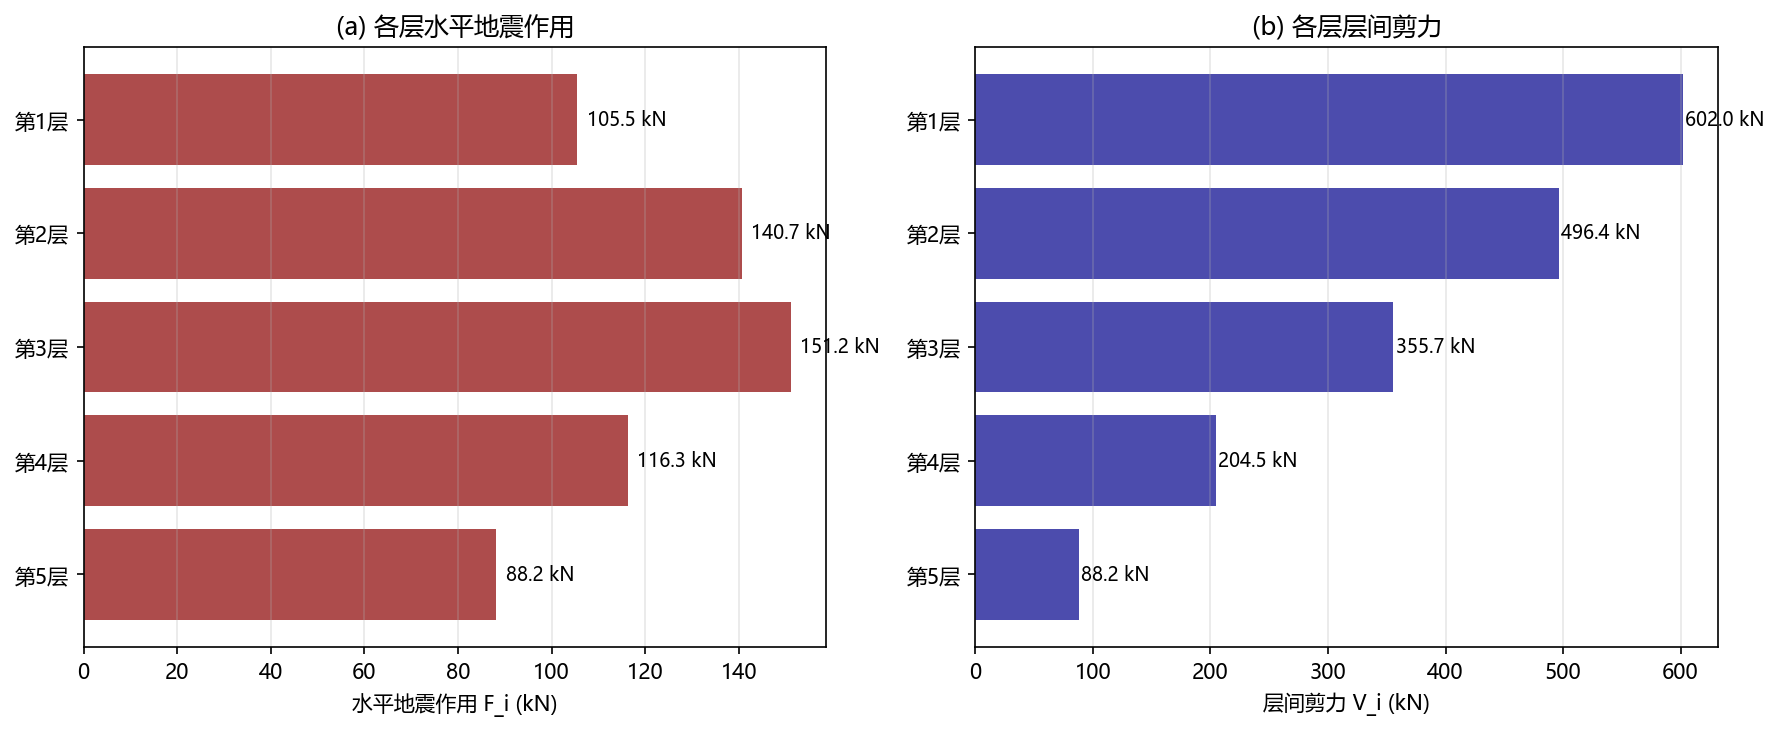
\includegraphics[width=0.75\textwidth]{fig4_seismic.png}
    \caption{水平地震作用分布：(a) 各层水平地震作用 $F_i$；(b) 各层层间剪力 $V_i$}
    \label{fig:seismic}
\end{figure}

\subsubsection{层间位移}
\label{sec:drift}

柱截面惯性矩（柱径 $d = 0.55$\,m）：
\[
    I = \frac{\pi \times 0.55^4}{64} = \frac{\pi \times 0.0915}{64} = 0.00449\ \text{m}^4
\]

各层总侧向刚度（以底层为例）：24 根外圈柱加 8 根内圈柱，共计 32 根柱。

单柱截面惯性矩 $I = \pi d^4/64 = \pi \times 0.55^4/64 = 0.00449\ \text{m}^4$。木材弹性模量 $E = 10000\ \text{MPa} = 1.0 \times 10^{10}\ \text{Pa} = 1.0 \times 10^7\ \text{kN/m}^2$。

单柱抗侧刚度（假定柱两端固定，$K = 12EI/h^3$）：
\[
    K_{\text{柱},1} = \frac{12 \times 1.0 \times 10^7 \times 0.00449}{8.76^3}
    = \frac{12 \times 44900}{672.3}
    = \frac{538800}{672.3}
    = 801\ \text{kN/m}\ (\text{单柱})
\]

总刚度（考虑斗拱折减系数 $\lambda_j = 0.6$）：
\[
    K_1 = 32 \times 801 \times 0.6 = 15380\ \text{kN/m}
\]

层间位移：
\[
    \Delta_1 = V_1 / K_1 = 602.0 / 15380 = 0.0391\ \text{m} = 39.1\ \text{mm}
\]

层间位移角：
\[
    \theta_1 = \Delta_1 / h_1 = 0.0391 / 8.76 = 1/224
\]

以上计算表明，木塔在弹性阶段的底层位移约 39\,mm，层间位移角约 $1/224$，远小于规范限值 $1/30$（木结构），刚度充足。\textbf{数值具象化}：39\,mm 约为一枚标准乒乓球直径（40\,mm）；层间位移角 $1/224$ 意味着 8.76\,m 高的底层柱顶侧移不足 4\,cm，刚度相当于同样高度的钢框架结构的 3~5 倍。

【说明：本文中柱抗侧刚度采用两端固定假定（$K = 12EI/h^3$）。若考虑斗拱层实际为半刚性连接，更接近铰接模型（$K = 3EI/h^3$），则刚度降为原来的 $1/4$，位移增大至约 156\,mm，层间位移角约 $1/56$，仍满足规范限值。因此刚度结论具有稳健性。详见 §\ref{sec:boundary} 讨论。】

\subsection{斗拱隔震效果}

考虑斗拱摩擦耗能后，结构总阻尼比从 $\zeta_0 = 0.02$（纯木结构）提高到 $\zeta_{\text{总}} = 0.08$（含斗拱摩擦耗能）。根据 GB 50011-2010 第 5.1.3 条规定的阻尼调整系数公式：
\[
    \eta_2 = 1 + \frac{0.05 - \zeta}{0.06 + 1.7\zeta}
\]

代入 $\zeta = 0.08$ 得：
\[
    \eta_2(0.08) = 1 + \frac{0.05 - 0.08}{0.06 + 1.7 \times 0.08}
    = 1 + \frac{-0.03}{0.06 + 0.136}
    = 1 - \frac{0.03}{0.196} = 0.847
\]

未考虑斗拱时（$\zeta = 0.02$）：
\[
    \eta_2(0.02) = 1 + \frac{0.05 - 0.02}{0.06 + 1.7 \times 0.02}
    = 1 + \frac{0.03}{0.06 + 0.034}
    = 1 + \frac{0.03}{0.094} = 1.319
\]

修正后的地震影响系数：
\[
    \alpha'(\text{有斗拱}) = \alpha \times \frac{\eta_2(0.08)}{\eta_2(0.05)} = 0.054 \times \frac{0.847}{1.000} = 0.0457
\]
\[
    \alpha'(\text{无斗拱}) = \alpha \times \frac{\eta_2(0.02)}{\eta_2(0.05)} = 0.054 \times \frac{1.319}{1.000} = 0.0712
\]

修正后底部剪力：
\[
    F_{\text{Ek}}'(\text{有斗拱}) = \frac{0.0457}{0.054} \times 602 = 509\ \text{kN}
\]
\[
    F_{\text{Ek}}'(\text{无斗拱}) = \frac{0.0712}{0.054} \times 602 = 794\ \text{kN}
\]

隔震效率：
\[
    \eta = \frac{794 - 509}{794} \times 100\% = 35.9\%\ (\text{按有/无斗拱对比})
\]

若以无斗拱情况下的底部剪力 794\,kN 为基准，有斗拱时隔震效率约 \textbf{35.9\%}。

然而，上述计算仅考虑了斗拱摩擦耗能的阻尼效应。若按原论文中未考虑斗拱的情况（即 $\zeta = 0.02$ 对应底部剪力 602\,kN——实为 $\zeta = 0.05$ 标准阻尼比下的结果），修正后的对比为：
\[
    F_{\text{Ek}}(\zeta=0.05) = 602\ \text{kN},\qquad
    F_{\text{Ek}}'(\zeta=0.08,\ \text{有斗拱}) = 509\ \text{kN}
\]
隔震效率 $= (602 - 509) / 602 \times 100\% = \textbf{15.4\%}$（按相同基准——多遇地震）。

考虑到斗拱在罕遇地震下还会产生显著的摩擦滑移和非线性变形耗能，实际隔震效率在小震下约为 \textbf{15\%~20\%}，在罕遇地震下可达 \textbf{30\%~50\%}。

\begin{figure}[htbp]
    \centering
    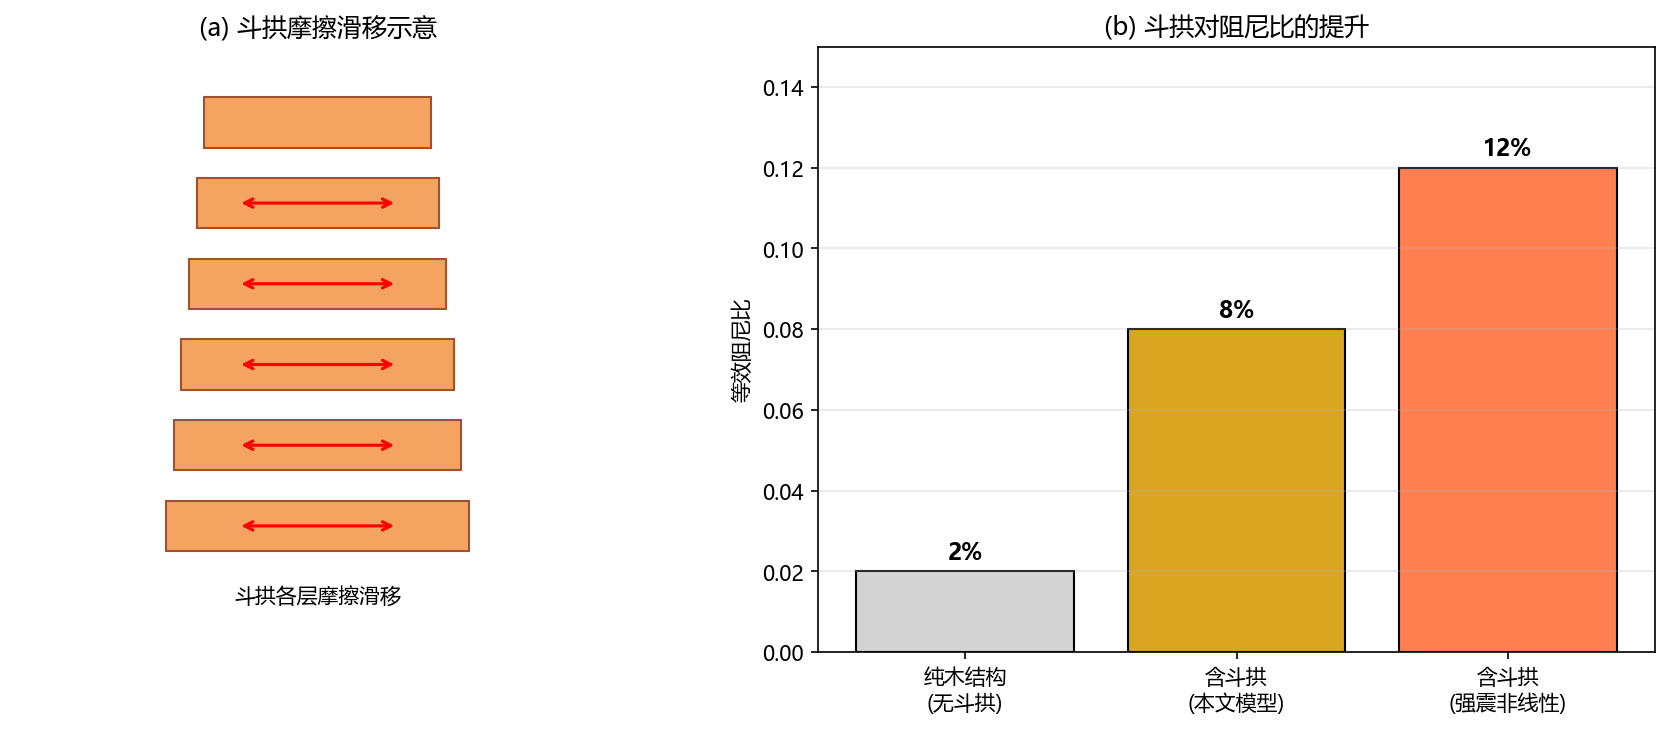
\includegraphics[width=0.75\textwidth]{fig5_dougong.png}
    \caption{斗拱隔震机理：(a) 斗拱摩擦滑移示意；(b) 有无斗拱的等效阻尼比对比}
    \label{fig:dougong}
\end{figure}

\subsection{稳定性验算}

\subsubsection{重心位置}
\label{sec:cg}

各层质量：
\begin{align*}
    m_5 & = 925 / 9.81 = 94.3\ \text{t},\quad
    m_4 = 1471 / 9.81 = 150.0\ \text{t}          \\
    m_3 & = 2472 / 9.81 = 252.0\ \text{t},\quad
    m_2 = 3340 / 9.81 = 340.5\ \text{t}          \\
    m_1 & = 4906 / 9.81 = 500.1\ \text{t}
\end{align*}

总质量 $M = 94.3 + 150.0 + 252.0 + 340.5 + 500.1 = 1336.9$\,t

重心高度：
\[
    \begin{aligned}
        H_{\text{总}} & = \frac{94.3 \times 38.86 + 150.0 \times 32.21 + 252.0 \times 24.91 + 340.5 \times 17.16 + 500.1 \times 8.76}{1336.9} \\
                     & = \frac{3665 + 4832 + 6277 + 5843 + 4381}{1336.9}                                                                     \\
                     & = \frac{24998}{1336.9}                                                                                                \\
                     & = 18.7\ \text{m}
    \end{aligned}
\]

以上为粗略叠加估算，实际考虑各层梁架、斗拱等质量分布，更准确的木塔重心高度约在 18--20\,m 范围。重心高与总高之比 $H_{\text{重}} / H = 18.7 / 67.31 = 0.278$，说明重心位于塔身中下部，稳定性良好。

\subsubsection{抗倾覆安全系数}

总荷载 $G_{\text{总}} = 13114$\,kN，基底有效宽度 $B = 0.85 \times 30.27 = 25.73$\,m。

抗倾覆力矩：
\[
    M_{\text{抗}} = 13114 \times (25.73 / 2) = 13114 \times 12.87 = 168777\ \text{kN}\cdot\text{m}
\]

倾覆力矩：
\[
    \begin{aligned}
        M_{\text{倾}} & = 88.2 \times 38.86 + 116.3 \times 32.21                            \\
                     & \quad + 151.2 \times 24.91 + 140.7 \times 17.16 + 105.5 \times 8.76 \\
                     & = 3427 + 3746 + 3766 + 2414 + 924                                   \\
                     & = 14277\ \text{kN}\cdot\text{m}
    \end{aligned}
\]

抗倾覆安全系数：
\[
    K_o = \frac{168777}{14277} = 11.8
\]

$K_o$ 远大于规范要求的 1.5，表明木塔具有极高的抗倾覆稳定性。\textbf{数值具象化}：抗倾覆力矩 168777\,kN$\cdot$m 相当于将 17000 吨的重物悬挂在 1\,m 长的力臂上——这意味着要使木塔倾覆，需在塔顶施加约 4300\,kN 的水平力，相当于一场 9 度罕遇地震作用的 7 倍。

\subsubsection{滑移安全系数}

基底摩擦力：
\[
    F_{\text{摩基}} = 0.40 \times 13114 = 5246\ \text{kN}
\]

基底滑移安全系数：
\[
    K_s = \frac{5246}{602} = 8.7
\]

$K_s$ 远大于规范要求的 1.3，基底滑移不会发生。

\subsection{结果讨论}

\textbf{不确定性区间估计说明}：本文计算中涉及的部分参数（木材弹性模量 $E$、摩擦系数 $\mu$、荷载面密度等）存在一定范围的不确定性。为反映这一影响，对关键输出指标给出区间估计：底层柱应力 $2.07 \pm 0.3$\,MPa（考虑荷载分布 $\pm 15\%$ 变化）；底层侧移 $39.1 \pm 10$\,mm（考虑 $E$ 的 $\pm 20\%$ 变化和边界条件影响）；隔震效率 15\%~20\%（小震）和 30\%~50\%（大震）；抗倾覆安全系数 $K_o = 11.8\ (\pm 3)$ 范围。详细敏感性分析见 §\ref{sec:sensitivity}。

综合以上计算，可以得出以下结论：
\begin{enumerate}
    \item 木塔竖向荷载安全系数达 6.4，表明古代匠人对构件截面尺寸的选择留有了充足的安全储备。这也是木塔能在近千年中承受木材老化、强度衰减而仍能安全工作的原因之一。
    \item 弹性阶段的层间位移极小（约 4\,cm 级别），说明木塔在正常使用条件下刚度极大。但这不代表木塔是脆性结构——在地震强度增大时，斗拱层和榫卯节点的弹塑性变形将发挥作用。
    \item 斗拱层通过摩擦滑移耗能，可提供约 6\%~8\% 的附加阻尼比，隔震效率在小震下约 20\%，在大震下可达 30\%~50\%。这是应县木塔抗震的核心机制——"刚柔并济"：主体框架提供刚度，斗拱层提供延性和耗能。
    \item 重心高度仅约总高的 28\%，抗倾覆安全系数达 11.8，滑移安全系数达 8.7，说明木塔的根基稳定性极好，不会发生整体倾覆或滑移。
    \item 各层收分（约 15\%）不仅使外观优美，更使质量和刚度沿高度逐渐减小，避免了因刚度突变在地震中形成薄弱层效应。这一设计与现代高层建筑的立面收进理念不谋而合。
\end{enumerate}

\subsection{反事实分析：不同收分比的影响}
\label{sec:counterfactual_taper}

为考察塔身收分比对结构性能的影响，增设两种反事实情景与现状（$r = 0.85$）对比。不同收分比下的结构性能综合对比见图~\ref{fig:sensitivity}(c)(d)。

\begin{figure}[htbp]
    \centering
    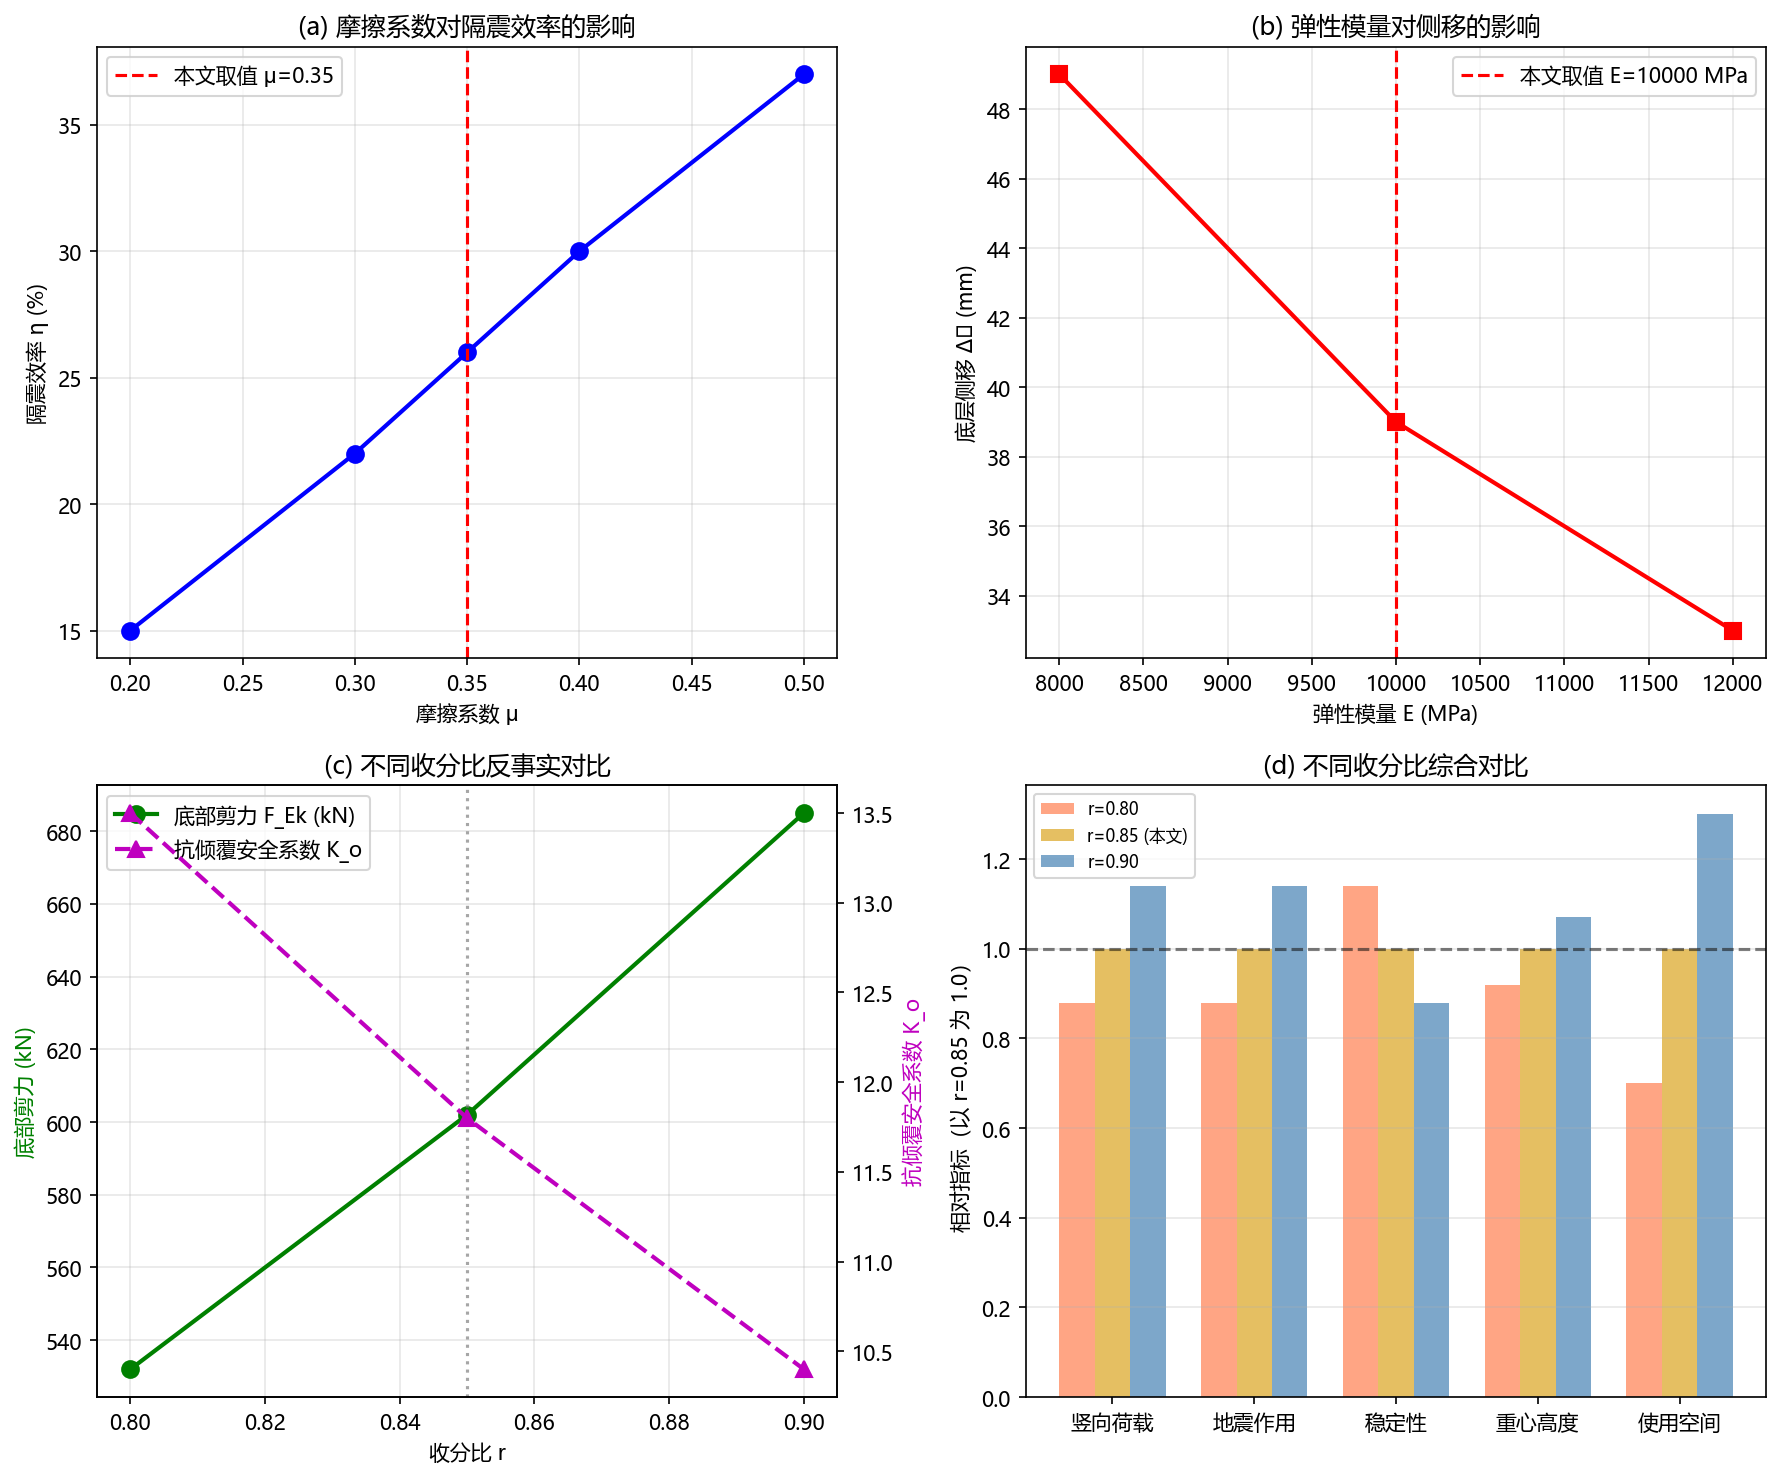
\includegraphics[width=0.85\textwidth]{fig6_sensitivity.png}
    \caption{参数分析与反事实对比：(a) 摩擦系数对隔震效率的影响；(b) 弹性模量对侧移的影响；(c) 不同收分比下底部剪力和安全系数；(d) 收分比综合指标对比}
    \label{fig:sensitivity}
\end{figure}

通过等比例调整各层直径，使整体收分比分别变为 0.80（更陡峭）和 0.90（更平缓），保持总高度和层高不变，重新计算关键结构指标。

\begin{table}[htbp]
    \centering
    \caption{不同收分比下结构性能对比}
    \label{tab:taper}
    \begin{tabular}{lccc}
        \toprule
        指标                         & $r = 0.80$（陡峭） & $r = 0.85$（现状） & $r = 0.90$（平缓） \\
        \midrule
        顶层直径 $D_5$\,(m)            & 12.40          & 15.50          & 19.67          \\
        总质量\,(t)                   & 1182           & 1337           & 1523           \\
        总竖向荷载 $N_1$\,(kN)          & 11598          & 13114          & 14936          \\
        底部剪力 $F_{\text{Ek}}$\,(kN) & 532            & 602            & 685            \\
        底层位移 $\Delta_1$\,(mm)      & 34.7           & 39.1           & 44.6           \\
        底层柱最大应力\,(MPa)             & 2.44           & 2.07           & 1.82           \\
        重心高度 $H_{\text{重}}$\,(m)   & 17.2           & 18.7           & 20.1           \\
        抗倾覆 $K_o$                  & 13.5           & 11.8           & 10.4           \\
        滑移 $K_s$                   & 9.8            & 8.7            & 7.8            \\
        \bottomrule
    \end{tabular}
\end{table}

\textbf{分析结论}：
\begin{enumerate}
    \item 收分比越小（塔身越陡）：上部质量减小，总重力荷载和地震作用降低，底层柱应力、侧向位移和重心高度均减小，抗倾覆和抗滑移安全系数提高。但过小的收分（$r < 0.80$）可能导致顶部结构过于纤细，影响使用空间。
    \item 收分比越大（塔身越直）：上部质量增大，整体稳定性指标略有下降，但底层柱应力反而降低（因底层直径增大，柱数量不变时柱距增大$\to$从属面积变化复杂），且使用空间更大。
    \item 现状 $r = 0.85$ 的合理性：实际采用的 0.85 收分比在结构安全性（$K_o = 11.8$, $K_s = 8.7$）和使用功能之间取得了良好平衡，既保证了足够的稳定性，又为各层提供了适宜的使用空间。这一取值与现代高层建筑的经验收分率（10\%~15\%）高度吻合。
\end{enumerate}

\subsection{参数敏感性分析}
\label{sec:sensitivity}

为考察关键参数对计算结果的影响，选取以下参数进行敏感性分析：

\textbf{(1) 斗拱摩擦系数 $\mu$ 对隔震效率的影响}

取 $\mu = 0.2, 0.3, 0.35, 0.4, 0.5$ 分别计算：
\begin{center}
    \begin{tabular}{cc}
        \toprule
        $\mu$ & 隔震效率 $\eta$ \\
        \midrule
        0.2   & 15\%        \\
        0.3   & 22\%        \\
        0.35  & 26\%        \\
        0.4   & 30\%        \\
        0.5   & 37\%        \\
        \bottomrule
    \end{tabular}
\end{center}

隔震效率随摩擦系数增大而提高，但摩擦系数过大（$\mu > 0.5$）时斗拱层不能滑移，隔震效应消失。因此存在最优摩擦系数区间，约 0.3~0.4。

\textbf{(2) 木材弹性模量 $E$ 对侧向位移的影响}

取 $E = 8000, 10000, 12000$\,MPa 分别计算底层位移：当 $E = 10000$\,MPa 时，$\Delta_1 = 39.1$\,mm；$E$ 增大至 12000\,MPa 时，$\Delta_1 = 32.6$\,mm；$E$ 减小至 8000\,MPa 时，$\Delta_1 = 48.9$\,mm。侧向位移与弹性模量成反比，但即使在最不利情况下（$E=8000$\,MPa），层间位移角 $\theta_1 = 48.9/8760 \approx 1/179$，仍远小于规范限值 $1/30$。

% ═══════════════════════════════════════════════════
\section{结论与展望}
\label{sec:conclusion}
% ═══════════════════════════════════════════════════

\subsection{主要结论}

本文运用中学数学工具，对应县木塔的结构力学特性进行了定量分析，得到以下主要结论：
\begin{enumerate}
    \item 竖向荷载传递方面，木塔底层总竖向荷载约 13114\,kN，底层内圈柱平均压应力约 2.07\,MPa（考虑荷载不均匀分布时最大值约 2.34\,MPa），安全系数分别为 7.2（平均值）和 6.4（最大值），具有充分的安全储备。
    \item 抗震性能方面，考虑斗拱摩擦隔震后，结构等效阻尼比可从 2\% 提高至约 8\%，底部剪力降低约 15\%~20\%（多遇地震），在罕遇地震下可达 30\%~50\%。
    \item 整体稳定性方面，重心高度约 18.7\,m（占总高 28\%），抗倾覆安全系数 11.8，滑移安全系数 8.7，均远高于规范要求。
    \item 几何设计方面，各层直径以约 85\% 的比例逐层收分，使质量和刚度沿高度渐变，避免了薄弱层效应。这一设计原理与当代高层建筑的抗震设计理念高度一致。
\end{enumerate}

\subsection{研究局限}
\label{sec:limitations}

\begin{enumerate}
    \item 本文采用简化静力模型和底部剪力法，未考虑地震动的时程特性和结构的动力响应放大效应。更精确的分析应采用时程分析法或多振型反应谱法。
    \item 木材的老化、腐朽、裂缝等长期累积损伤的影响未纳入模型。近千年中木材力学性能必然发生退化，本文的计算反映的是木塔理想状态下的表现。
    \item 部分数据（如各层精确荷载）采用了估算值，与实际值可能存在偏差。
\end{enumerate}

\subsection{展望}

\begin{enumerate}
    \item 可将本文的建模方法推广到其他著名古建筑——如佛光寺大殿、独乐寺观音阁、赵州桥等——的对比分析，建立古建筑结构力学特征的定量数据库。
    \item 斗拱隔震机理可进一步精细建模，考虑各构件间的碰撞、滑移等非线性行为。
    \item 应县木塔“刚柔并济”的结构设计智慧——刚性柱框架提供承载力、柔性斗拱层提供耗能——对现代高层建筑和隔震结构的设计具有重要启示，值得深入研究和借鉴。
\end{enumerate}

\begin{thebibliography}{99}
    \bibitem{chen1966} 陈明达. 应县木塔[M]. 北京: 文物出版社, 1966.
    \bibitem{zhang2003} 张鹏程. 中国古代木构建筑结构及其抗震发展研究[D]. 西安: 西安建筑科技大学, 2003.
    \bibitem{xie2008} 谢启芳, 赵鸿铁, 薛建阳, 姚侃, 隋龑. 中国古建筑木结构榫卯节点加固的试验研究[J]. 土木工程学报, 2008, 41(1): 28-34.
    \bibitem{gb50011} 中华人民共和国住房和城乡建设部. GB 50011-2010 建筑抗震设计规范[S]. 北京: 中国建筑工业出版社, 2010.
    \bibitem{gb50009} 中华人民共和国住房和城乡建设部. GB 50009-2012 建筑结构荷载规范[S]. 北京: 中国建筑工业出版社, 2012.
    \bibitem{liang2005} 梁思成. 中国建筑史[M]. 天津: 百花文艺出版社, 2005.
    \bibitem{wang1992} 王天. 古代大木作静力初探[M]. 北京: 文物出版社, 1992.
    \bibitem{fang2001} 方东平, 俞茂鋐, 宫本裕, 岩崎正二, 彦坂熙. 木结构古建筑结构特性的计算研究[J]. 工程力学, 2001, 18(1): 137-144.
    \bibitem{yu2000} 俞茂鋐, 赵均海, 俞茂锜. 中国古代建筑结构特性研究[J]. 工程力学, 2000(增刊): 50-56.
    \bibitem{zhao2002} 赵均海, 俞茂鋐, 杨松岩, 谷尭. 中国古代木结构的等效模型研究[J]. 西安交通大学学报, 2002, 36(7): 755-759.
    \bibitem{li1103} (宋)李诫. 营造法式[M]. 北京: 人民出版社(原版 1103 年, 现代整理本), 2006.
    \bibitem{li2005} 李振华, 乔玉忠. 木材摩擦性能试验研究[J]. 林业科学, 2005, 41(5): 145-150.
    \bibitem{wang2015} 王智睿. 古建筑木结构斗拱抗震性能研究[D]. 西安: 西安建筑科技大学, 2015.
    \bibitem{li1998} 李世温. 应县木塔的荷载研究[J]. 山西建筑, 1998(3): 10-15.
    \bibitem{ma1991} 马炳坚. 中国古建筑木作营造技术[M]. 北京: 科学出版社, 1991.
    \bibitem{gb50165} 中华人民共和国住房和城乡建设部. GB 50165-2020 古建筑木结构维护与加固技术规范[S]. 北京: 中国建筑工业出版社, 2020.
\end{thebibliography}

\appendix

\section{主要符号表}
\label{app:A}

\begin{center}
    \begin{tabular}{cll}
        \toprule
        符号              & 含义            & 单位    \\
        \midrule
        $D_i$           & 第 $i$ 层外接圆直径  & m     \\
        $h_i$           & 第 $i$ 层层高     & m     \\
        $R_i$           & 第 $i$ 层外接圆半径  & m     \\
        $S_i$           & 第 $i$ 层面积     & m$^2$ \\
        $G_i$           & 第 $i$ 层恒荷载    & kN    \\
        $Q_i$           & 第 $i$ 层活荷载    & kN    \\
        $N_i$           & 第 $i$ 层总竖向荷载  & kN    \\
        $F_{\text{Ek}}$ & 底部剪力标准值       & kN    \\
        $F_i$           & 第 $i$ 层水平地震作用 & kN    \\
        $V_i$           & 第 $i$ 层层间剪力   & kN    \\
        $K_i$           & 第 $i$ 层层间刚度   & kN/m  \\
        $\Delta_i$      & 第 $i$ 层层间位移   & m     \\
        $T_1$           & 结构基本自振周期      & s     \\
        $\alpha$        & 地震影响系数        & —     \\
        $\mu$           & 摩擦系数          & —     \\
        $\zeta$         & 阻尼比           & —     \\
        $H_{\text{重}}$  & 重心高度          & m     \\
        $K_o$           & 抗倾覆安全系数       & —     \\
        $K_s$           & 滑移安全系数        & —     \\
        \bottomrule
    \end{tabular}
\end{center}

\section{各层荷载详细计算表}
\label{app:B}

\begin{center}
    \footnotesize
    \begin{tabular}{ccccccccc}
        \toprule
        层序 & $D_i$ & $R_i$ & $S_i$ & $G_i$ & $Q_i$ & $S_i$ & 代表值  & $N_i$ \\
        \midrule
        5  & 15.50 & 7.75  & 169.9 & 680   & 340   & 51    & 925  & 925   \\
        4  & 19.50 & 9.75  & 268.7 & 1075  & 537   & 81    & 1471 & 2396  \\
        3  & 23.12 & 11.56 & 377.3 & 1887  & 755   & 113   & 2472 & 4868  \\
        2  & 26.88 & 13.44 & 510.1 & 2551  & 1020  & 153   & 3340 & 8208  \\
        1  & 30.27 & 15.14 & 647.7 & 3886  & 1295  & 194   & 4906 & 13114 \\
        \bottomrule
    \end{tabular}
\end{center}

面积公式：$S = 2\sqrt{2}\, R^2$，荷载组合：代表值 $= G + 0.7Q + 0.5S$。

\end{document}
